\begin{footnotesize}
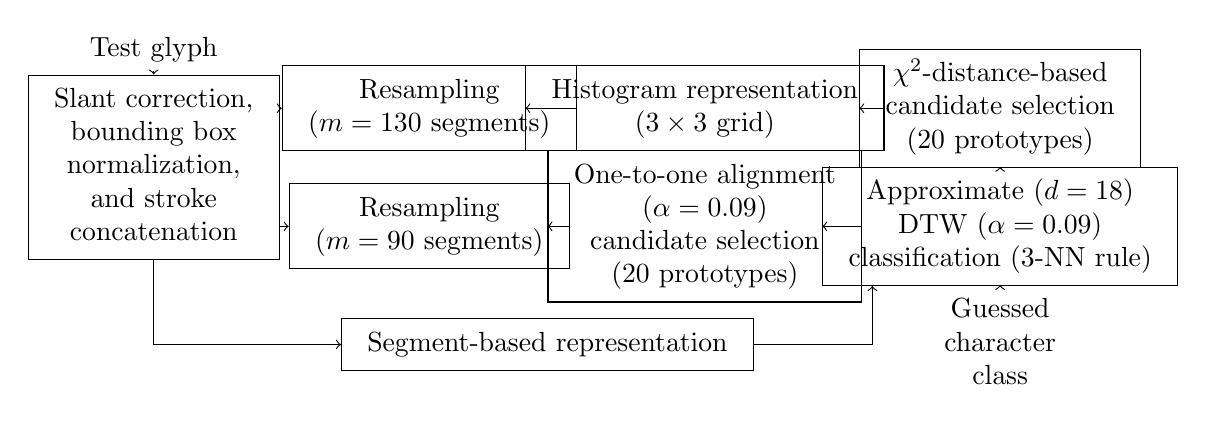
\begin{tikzpicture}

  \draw (2,0) node [draw,shape=rectangle] (prepro)
  {\begin{tabular}{c}Slant correction,\\bounding box\\normalization,\\and stroke\\concatenation\end{tabular}};
  
  \draw (5.5,-.75) node [draw,shape=rectangle] (preproA)
  {\begin{tabular}{c}Resampling\\($m=90$ segments)\end{tabular}};

  \draw (9,-.75) node [draw,shape=rectangle] (preproA2)
  {\begin{tabular}{c}One-to-one alignment\\($\alpha=0.09$)\\candidate selection\\($20$ prototypes)\end{tabular}};

  \draw (5.5,.75) node [draw,shape=rectangle] (preproB)
  {\begin{tabular}{c}Resampling\\($m=130$ segments)\end{tabular}};

  \draw (9,.75) node [draw,shape=rectangle] (preproB2)
  {\begin{tabular}{c}Histogram representation\\($3\times{}3$ grid)\end{tabular}};

  \draw (12.75,.75) node [draw,shape=rectangle] (preproB3)
  {\begin{tabular}{c}$\chi^2$-distance-based\\candidate selection\\($20$ prototypes)\end{tabular}};

  \draw (12.75,-.75) node [draw,shape=rectangle] (DTW)
  {\begin{tabular}{c}Approximate ($d=18$)\\DTW ($\alpha=0.09$)\\classification ($3$-NN rule)\end{tabular}};

  \draw (7,-2.25) node [draw,shape=rectangle] (ptseg)
  {\begin{tabular}{c}Segment-based representation\end{tabular}};

  \draw (12.75,-2.25) node [shape=rectangle] (out)
  {\begin{tabular}{c}Guessed\\character\\class\end{tabular}};

  \draw (2,1.5) node [shape=rectangle] (glyph)
  {Test glyph};

  \draw[->] (glyph.south) -- (prepro.north);
  \draw[->] (prepro.east) |- (preproA);
  \draw[->] (preproA.east) -- (preproA2.west);
  \draw[->] (prepro.east) |- (preproB);
  \draw[->] (preproB.east) -- (preproB2.west);
  \draw[->] (preproB2.east) -- (preproB3.west);
  \draw[->] (preproB3.south) -- (DTW.north);
  \draw[->] (preproA2.east) -- (DTW.west);
  \draw[->] (DTW.south) -- (out.north);
  \draw[->] (prepro.south) |- (ptseg.west);
  \draw[->] (ptseg.east) -| (DTW.205);

\end{tikzpicture}
\end{footnotesize}
%%% Local Variables: 
%%% mode: latex
%%% TeX-master: t
%%% End: 
